\section{文件管理}

\begin{frame}[fragile]{CH6 文件管理}
  \begin{easylist} \easyitem
    & 6.1 文件和文件系统
    & 6.2 文件的逻辑结构
    & 6.3 外存分配方式 
    & 6.4 目录管理
    & 6.5 文件存储空间的管理
    & 6.6 文件共享与文件保护
    & 6.7 数据一致性控制
  \end{easylist}
  TODO: 增加HDF5文件格式介绍
\end{frame}


\subsection{6.1 文件和文件系统}
\begin{frame}[fragile]{6.1 文件和文件系统}
  \begin{easylist}
    & 重点
    && 文件、记录和数据项
    && 文件类型和文件系统模型
    && 文件操作
  \end{easylist}
\end{frame}


\begin{frame}[fragile]{6.1.1 文件、记录和数据项}
  \begin{easylist}
    & 1. 数据项
    && 基本的数据单位,用于描述一个对象的某种属性 
    \vspace{1cm}
    && (1) 基本数据项:数据名、数据类型
    && (2) 组合数据项:由基本数据项组成
  \end{easylist}
\end{frame}

\begin{frame}[fragile]{2. 记录}
  \begin{easylist}
    & 记录是一组相关数据项的集合,用于描述一个对象在某方面的属性。
    & 关键字是唯一能标志一个记录的数据项
  \end{easylist}
\end{frame}

\begin{frame}[fragile]{3. 文件}
  \begin{easylist}
    & 文件是指由创建者所定义的、具有文件名的一组相关元素的集合。可分为有结构文件和无结构文件两种
    && 在有结构的文件中,文件由若干个相关记录组成
    && 无结构文件则被看成是一个字符流
    && 文件在文件系统中是一个最大的数据单位,它描述了一个对象集,用户利用文件名访问文件
    && 文件具有属性:类型、长度、物理位置、建立时间
  \end{easylist}
\end{frame}

\begin{frame}[fragile]{文件、记录和数据项之间的层次关系}
  \begin{easylist}

  \end{easylist}
\end{frame}

\begin{frame}[fragile]{6.1.2 文件类型和文件系统模型}
  \begin{easylist}
    & 类型
    && 一、按用途分类:
    &&& 系统文件,用户文件,库文件。
    &&& (用户对以上三者的访问权限不同)
    && 二、按文件中的数据形式分类
    &&& 源,目标,可执行。
    && 三、按存取控制属性分类
    &&& X,R,R/W
  \end{easylist}
\end{frame}

\begin{frame}[fragile]{文件类型(续)}
  \begin{easylist}
    && 四、逻辑结构
    &&& (1)有结构(记录式)
    &&& (2)无结构(流式)
    && 五、物理安排
    &&& (1)顺序文件;数据(连续放)
    &&& (2)链接文件;
    &&& (3)索引文件;
    && 六、文件与目录文件
  \end{easylist}
\end{frame}

\begin{frame}[fragile]{文件系统模型}
  \begin{easylist}
    & 概念:文件和对文件进行操纵和管理的软件集合。
    && 三个层:文件(对象及属性), 文件操作, 文件访问接口
    & 一、对象及属性
    && (1)文件
    && (2)目录:用于方便用户(提供文件逻辑名来访问文件)和提高文件存取速度。
    && (3)物理存贮空间的管理:提高外存利用率和文件存取速度。
  \end{easylist}
\end{frame}

\begin{frame}[fragile]{文件系统模型}
  \begin{easylist}
    & 二、对对象操纵和管理的软件集合
    && 文件管理系统的核心部分,包括:文件存储空间的管理、文件目录的管理、将文件的逻辑地址转换为物理地址的机制、读写管理、共享与保护等
    & 三、文件系统接口
    && 命令接口:
    && 程序接口:系统调用
    && GUI接口
  \end{easylist}
\end{frame}

\begin{frame}[fragile]{文件系统模型}
  \begin{center}
    \begin{tikzpicture}[c/.style={draw, minimum height=1cm, minimum width=5cm, align=center, fill=red!10}]
      \draw[] node[c](b1) {对象及其属性} node[c, above=0 of b1] (b2) {对对象操纵和管理的\\软件集合 }
      node[c, above=0 of b2] (b3) {文件系统接口} node[above=0.5 of b3](b4) {用户(程序)};

      \draw[->, very thick] (b4) -- (b3);
      \draw[->, very thick] ($(b4.south)+(-0.5,0)$) -- ($(b3.north)+(-0.5,0)$);
      \draw[->, very thick] ($(b4.south)+(0.5,0)$) -- ($(b3.north)+(0.5,0)$);
    \end{tikzpicture}
  \end{center}
\end{frame}

\begin{frame}[fragile]{6.1.3 文件操作}
  \begin{easylist}
    & 一、对记录操作——类似数据库
    & 二、对文件操作:
    && 创/删/读/写/截断(清空)/设置指针
    && 文件粉碎机的原理…
    & 三、打开关闭操作
    && 打开:将文件的属性从外存拷贝到内存打开文件表的一个表目中,并将该表目的编号(索引)返回给用户
    & 四、其它
    && 更名、更改属性/所有者/权限…
  \end{easylist}
\end{frame}

\begin{frame}[fragile]{常用文件操作命令}
  \begin{easylist}
    & 创建文件:touch
    & 删除文件:rm
    & 读/写文件:cat test.txt
    & 编辑文件:vi
    & 更改名称:mv
    & 更改属性:chmod
  \end{easylist}
\end{frame}

\begin{frame}[fragile]{补充:Docker}
  
\includegraphics[width=0.8\textwidth]{figure/docker.png}
\end{frame}

\subsection{6.2 文件的逻辑结构}
\begin{frame}[fragile]{6.2 文件的逻辑结构}
  \begin{easylist}
    & 概念:用户所能观察和访问到的文件的数据结构组织,独立于物理特性,容易检索和修改。
    && (1) 文件的逻辑结构(File Logical Structure):又称文件组织
    && (2) 文件的物理结构,又称为文件的存储结构,是指文件在外存上的存储组织形式 
    & 无论是逻辑还是物理结构,都会影响到文件的检索速度
  \end{easylist}
\end{frame}

\begin{frame}[fragile]{6.2.1 逻辑结构类型}
  \begin{easylist}
    & 对文件逻辑结构的基本要求
    && 能提高检索速度
    && 便于修改
    && 降低文件存储费用:减少文件占用的存储空间,不要求大片连续的存储空间
  \end{easylist}
\end{frame}

\begin{frame}[fragile]{类型1:有结构文件}
  \begin{easylist}
    & 有结构文件:由一个以上的记录构成的文件,又称记录式文件
    & 分类:
    && 按记录长度
    &&& 定长记录
    &&& 变长记录
    && 按组织方式
    &&& 顺序文件
    &&& 索引文件
    &&& 索引顺序文件
  \end{easylist}
\end{frame}

\begin{frame}[fragile]{类型2:无结构文件}
  \begin{easylist}
    & 由字符流构成的文件,又称流式文件
    && 长度以字节为单位
    && 采用读写指针来指出下一个要访问的字符
    && 可以把流式文件看作是记录式文件的一个特例
    && 所有的文件都可以看作是流式文件
  \end{easylist}
\end{frame}


\begin{frame}[fragile]{文件组织原则}
  \begin{easylist}
    & 文件组织的原则
    && 访问快速
    && 易于修改
    && 节约存储空间
    && 维护简单
    && 可靠
    & 以上原则可能矛盾:
    && 节约空间,则需要尽量避免冗余
    && 而冗余可以提高数据访问速度,如索引。
    &   下面按照组织方式分别讨论顺序、索引和索引顺序文件
  \end{easylist}
\end{frame}

\begin{frame}[fragile]{6.2.2 顺序文件}
  \begin{easylist}
    & 1、逻辑记录的排序
    && 串结构:各记录之间的顺序与关键字无关
    && 顺序结构:指文件中的所有记录按关键字(词)排列
    \vspace{1cm}
    && 思考:哪种查找效率更高?
  \end{easylist}
\end{frame}

\begin{frame}[fragile]{2 对顺序文件的读/写操作}
  \begin{center}
    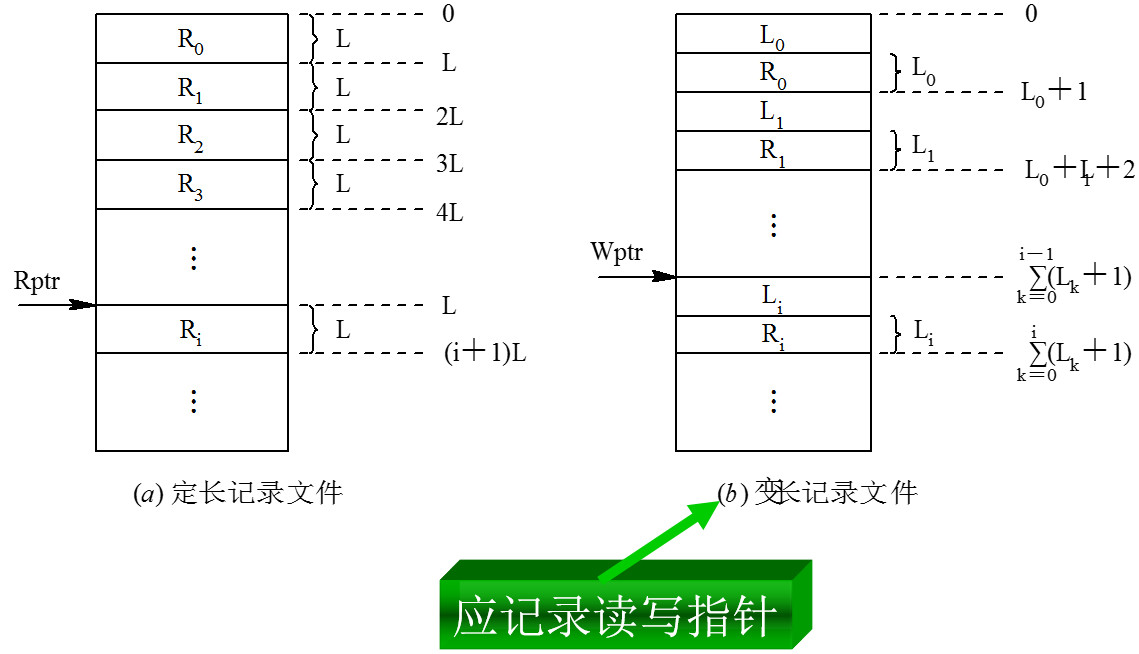
\includegraphics[width=0.8\textwidth]{figure/file/logic-sequence.jpg}
  \end{center}
\end{frame}

\begin{frame}[fragile]{3 顺序文件的优缺点}
  \begin{easylist}
    & 最佳应用场合,是在对诸记录进行批量存取时,即每次要读或写一大批记录
    & 顺序文件适合存储在磁带上
    & 交互应用的场合,当用户(程序)要求查找或修改单个记录时,顺序文件所表现出来的性能就可能很差,尤其是当文件较大时,情况更为严重
    & 如果想增加或删除一个记录,都比较困难
    && 为顺序文件配置一个运行记录文件(事务文件),把试图修改的信息记录下来,每隔一定时间与主文件合并,产生一个按关键字排序的新文件。
    && 类似于Hadoop的SequenceFile
  \end{easylist}
\end{frame}

\begin{frame}[fragile]{6.2.3 索引文件}
  \begin{easylist}
    & 定长记录文件第i个记录相对于第一个记录首址的地址:
    $$A_i = i \times L$$
    & 可变长度记录的文件假定在每个记录前用一个字节指明该记录的长度,则:

    && 对变长记录需要顺序访问前面的记录,难以实现直接存取
  \end{easylist}
\end{frame}

\begin{frame}[fragile]{变长记录存取问题}
  \begin{easylist}
    & 定长记录的顺序文件:顺序存取和直接存取都比较方便
    & 变长记录如何处理?
  \end{easylist}
\end{frame}

\begin{frame}[fragile]{索引表}
  \begin{easylist}
    & 为变长记录文件建立索引表,主文件的每个记录,在索引表中设有相应的表项,用于记录该记录的长度L及指向该记录的指针
    & 索引表本身是定长记录的顺序文件
  \end{easylist}
  \begin{center}
    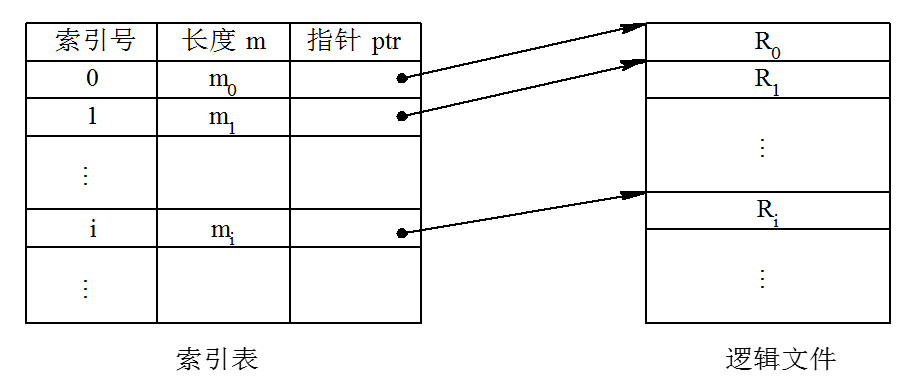
\includegraphics[width=0.8\textwidth]{figure/file/logic-index.jpg}
  \end{center}
\end{frame}

\begin{frame}[fragile]{索引表}
  \begin{easylist}
    & 索引文件的检索:关键字查找
    & 索引文件的使用场合:对信息处理的及时性要求较高
    & 增加了存储开销,除了主文件外,一般还有一个索引表文件
    \vspace{1cm}
    & 类似于Hadoop的MapFile
  \end{easylist}
\end{frame}

\begin{frame}[fragile]{6.2.4 索引顺序文件}
  \begin{easylist}
    & 记录分组,一组一个索引项 
  \end{easylist}
\begin{center}
    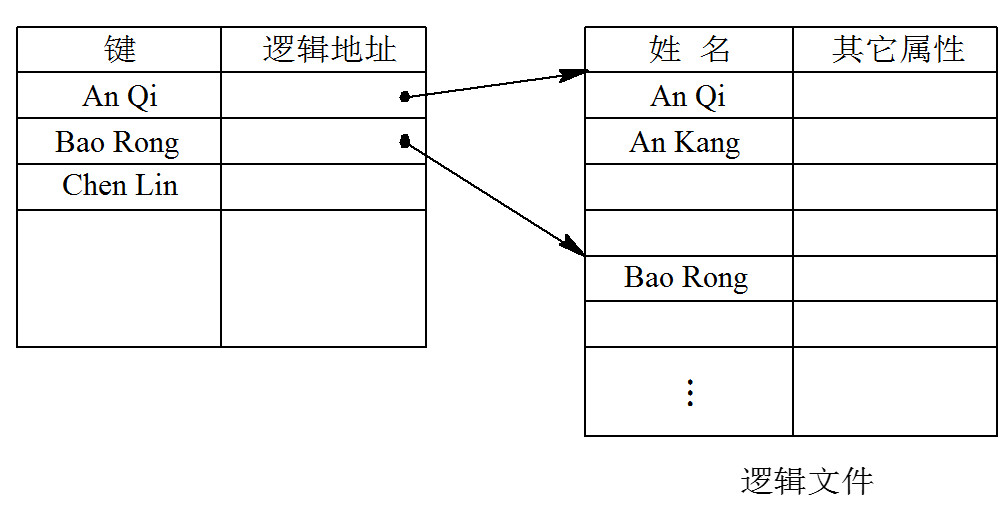
\includegraphics[width=0.8\textwidth]{figure/file/logic-index2.jpg}
  \end{center}
\end{frame}

\begin{frame}[fragile]{索引顺序文件}
  \begin{easylist}
    & 性能大大优于顺序文件
    & 记录较多时可以建立多级索引

    & E.g.
    && 汉语词典的首字二分查找法
  \end{easylist}
\end{frame}

\begin{frame}[fragile]{6.2.5 直接文件和哈希文件}
  \begin{easylist}
    & 1、直接文件
    && 根据给定的记录键值,直接获得指定记录的物理地址。即记录键值本身就决定了记录的物理地址。这种由记录键值到记录物理地址的转换被称为:
    &&& 键值转换(Key to address transformation)。
    && 组织直接文件的关键,在于用什么方法进行从记录值到物理地址的转换。
  \end{easylist}
\end{frame}

\begin{frame}[fragile]{哈希文件}
  \begin{easylist}
    & 2、哈希(Hash)文件 
    && 应用最为广泛的一种直接文件
    && 利用Hash函数将记录键值转换为相应记录的地址
  \end{easylist}

  \begin{center}
    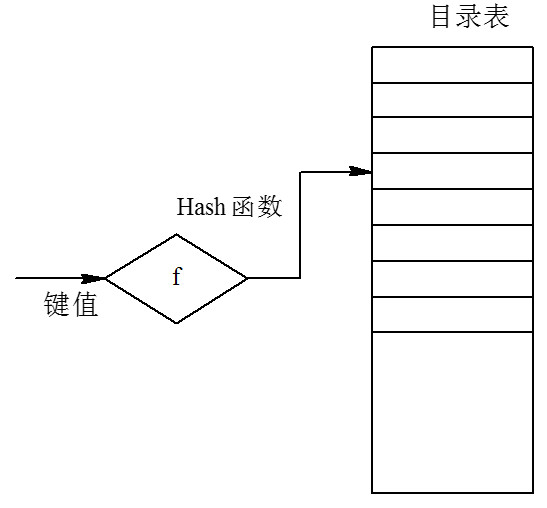
\includegraphics[width=0.5\textwidth]{figure/file/logic-hash.jpg}
  \end{center}
\end{frame}

\begin{frame}[fragile]{几种哈希函数的构造方法}
  \begin{easylist}
    & 平方取中法
    & 折叠法:如ISDN号码,可以折叠相加
    & 除留余数法:除数一般选择质数
    & 随机数法
  \end{easylist}
\end{frame}


\subsection{6.3 外存分配方式}
\begin{frame}[fragile]{6.3 外存分配方式}
  \begin{easylist}
    & 为文件分配外存时考虑的主要问题:
    && 提高外存空间的利用率
    && 提高文件访问速度
    & 常用的分配方法
    && 连续分配
    && 链接分配
    && 索引分配
  \end{easylist}
\end{frame}

\begin{frame}[fragile]{新创建文件的存储空间分配方法}
  \begin{easylist}
    & 预分配(preallocation):创建时(这时已知文件长度)一次分配指定的存储空间
    && 文件复制时的目标文件
    && 从网络下载文件
    & 动态分配(dynamic allocation):需要存储空间时才分配(创建时无法确定文件长度),如写入数据到文件。
  \end{easylist}
\end{frame}

\begin{frame}[fragile]{文件存储单位:簇(cluster)}
  \begin{easylist}
    & 文件的存储空间通常由多个分立的簇组成,而每个簇包含若干个连续的扇区(sector)。
    & 簇的大小
    && 两个极端:大到能容纳整个文件,小到一个外存存储块;
    && 簇较大:提高I/O访问性能,减小管理开销;但簇内碎片浪费问题较严重;
    && 簇较小:簇内的碎片浪费较小,特别是大量小文件时有利;但存在簇编号空间不够的问题(如FAT12、16、32);
  \end{easylist}
\end{frame}

\begin{frame}[fragile]{~}
  \begin{easylist}
    & 簇的分配方法:两种
    && 簇大小可变,其上限较大:I/O访问性能较好,文件存储空间的管理困难(类似于动态分区存储管理)
    && 簇大小固定,较小:文件存储空间使用灵活,但I/O访问性能下降,文件管理所需空间开销较大
    & 文件卷容量与簇大小的关系
    && 文件卷容量越大,若簇的总数保持不变即簇编号所需位数保持不变,则簇越大。缺点:簇内碎片浪费越多
    && 文件卷容量越大,若簇大小不变,则簇总数越多,相应簇编号所需位数越多。如簇编号长度为12、16、32二进制位,即构成FAT12、FAT16、FAT32。
  \end{easylist}
\end{frame}

\begin{frame}[fragile]{6.3.1 连续分配}
  \begin{center}
    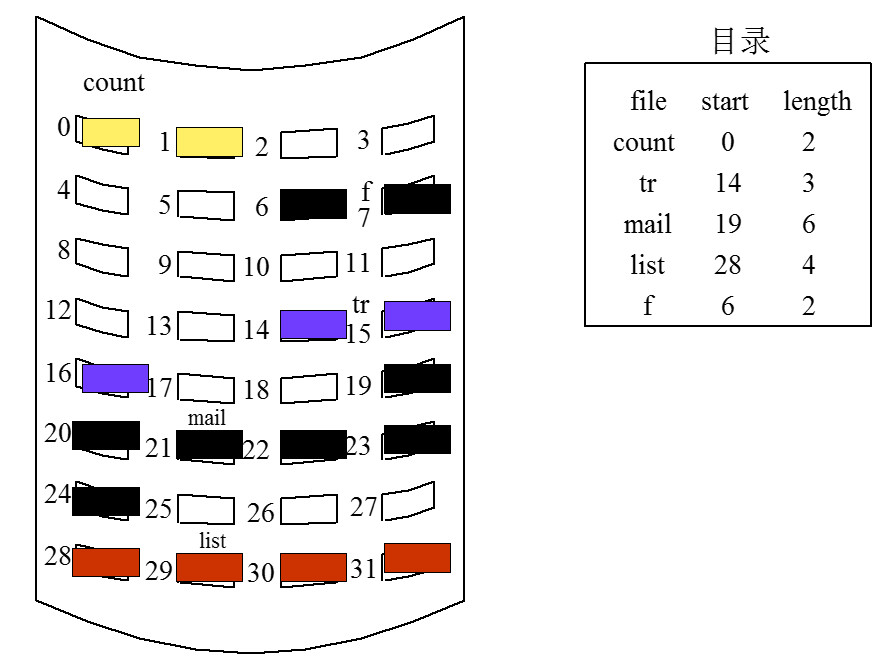
\includegraphics[width=0.8\textwidth]{figure/file/alloc-sequence.jpg}
  \end{center}
\end{frame}

\begin{frame}[fragile]{说明}
  \begin{easylist}
    & 连续分配方式形成的文件为顺序文件结构,此时的物理文件称为顺序文件
    & 保证了逻辑文件中的记录顺序与存储器中占用盘块的顺序的一致性
    \vspace{1cm}
    & ★紧凑问题
  \end{easylist}
\end{frame}

\begin{frame}[fragile]{连续分配的优缺点}
  \begin{easylist}
    & 优点
    && (1)顺序访问容易。 
    && (2)顺序访问速度快。
    & 缺点
    && (1)要求有连续的存储空间。 
    && (2)必须事先知道文件的长度。
  \end{easylist}
\end{frame}

\begin{frame}[fragile]{6.3.2 链接分配}
  \begin{easylist}
    & 在每个盘块上设置链接指针,将同属于一个文件的多个离散的盘块链接成一个链表——链接文件
    && 离散分配方式
    && 无需事先知道文件大小
    && 对文件的增、删、改非常方便 
  \end{easylist}
\end{frame}

\begin{frame}[fragile]{1.隐式链接}
  \begin{center}
    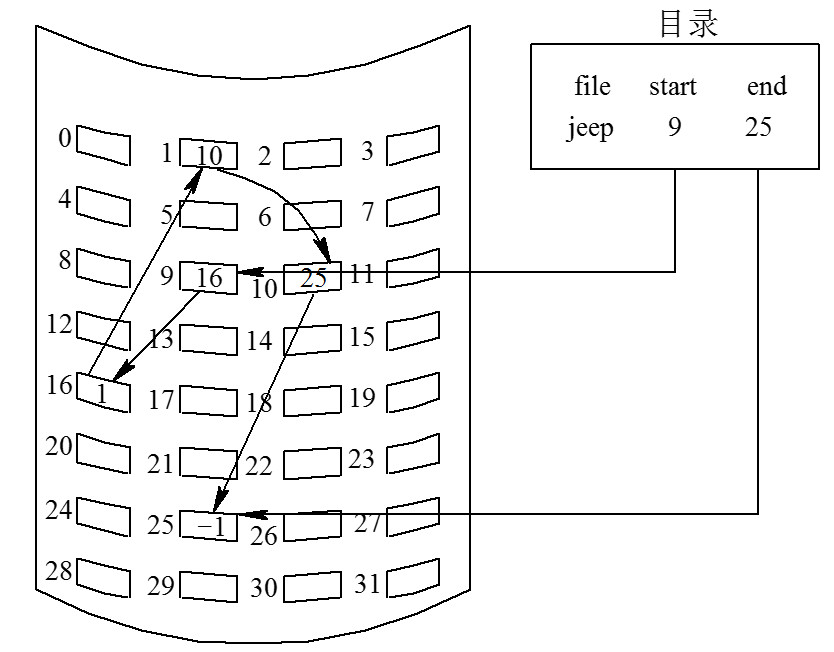
\includegraphics[width=0.8\textwidth]{figure/file/alloc-link.jpg}
  \end{center}
\end{frame}

\begin{frame}[fragile]{隐式链接分配的特点}
  \begin{easylist}
    & 只适合顺序访问
    & 可靠性差
  \end{easylist}
\end{frame}

\begin{frame}[fragile]{2.显式链接}
\begin{center}
    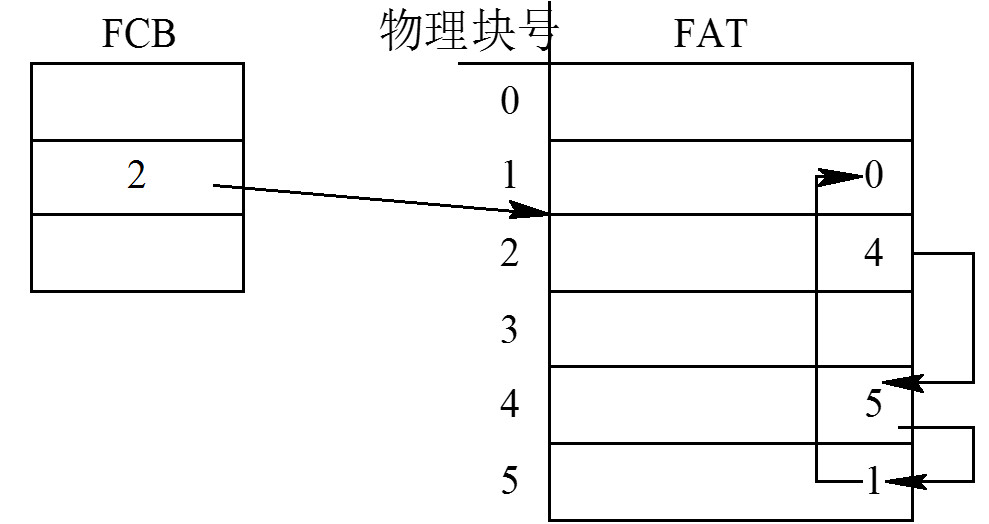
\includegraphics[width=0.8\textwidth]{figure/file/alloc-link-explict.jpg}
  \end{center}
  \begin{easylist}
    & 分配给文件的所有盘块号都放在表中,该表又称为文件分配表FAT, MS-DOS/Windows/OS2都采用了FAT
  \end{easylist}
\end{frame}

\begin{frame}[fragile]{2.显式链接}
  \begin{columns}[T]
    \begin{column}{0.6\textwidth}
      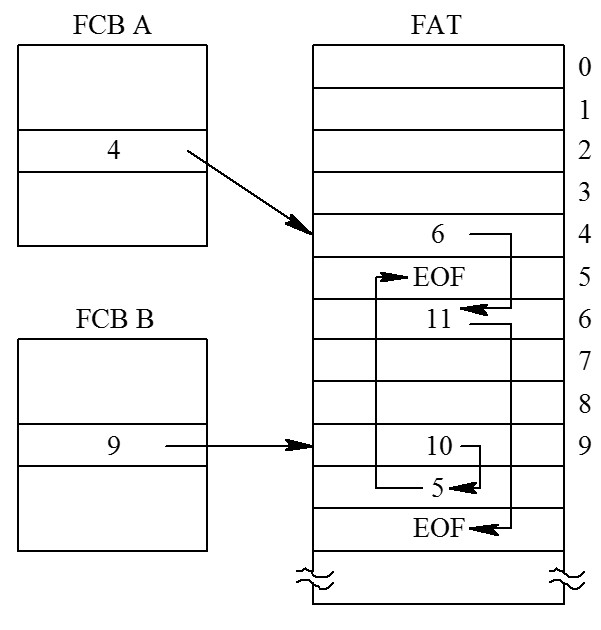
\includegraphics[width=0.8\textwidth]{figure/file/alloc-fat.jpg}
    \end{column}
    \begin{column}{0.4\textwidth}
      FAT在内存中,速度很快,整个系统一张FAT,FAT需要占用一定的内存空间 \\
      文件的初始指针保存在FCB中(什么是FCB?)
    \end{column}
  \end{columns}
\end{frame}

\begin{frame}[fragile]{6.3.3 索引分配}
  \begin{easylist}
    & 链接分配方式虽然解决了连续分配方式所存在的问题,但又出现了另外两个问题,即:
    && (1) 不能支持高效的直接存取。要对一个较大的文件进行直接存取,须首先在FAT中顺序地查找许多盘块号。
    && (2) FAT需占用较大的内存空间。 
  \end{easylist}
\end{frame}

\begin{frame}[fragile]{思想}
  \begin{easylist}
    & 打开文件时,只需要把该文件占用的盘块号调入内存即可,不需把整个FAT都调入
    & 把每个文件对应的盘块号集中到一起,为文件分配一个索引块,把分配给该文件的所有盘块号,都放在该索引块中。
  \end{easylist}
\end{frame}

\begin{frame}[fragile]{1. 单级索引分配}
  \begin{center}
    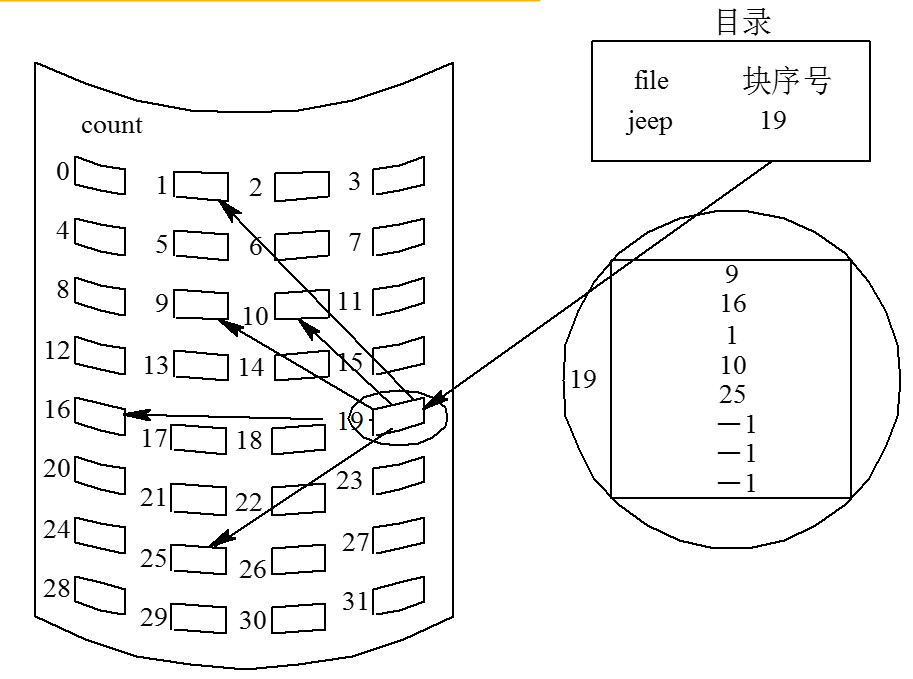
\includegraphics[width=0.8\textwidth]{figure/file/alloc-index.jpg}
  \end{center}
\end{frame}

\begin{frame}[fragile]{2. 多级索引分配}
  \begin{center}
    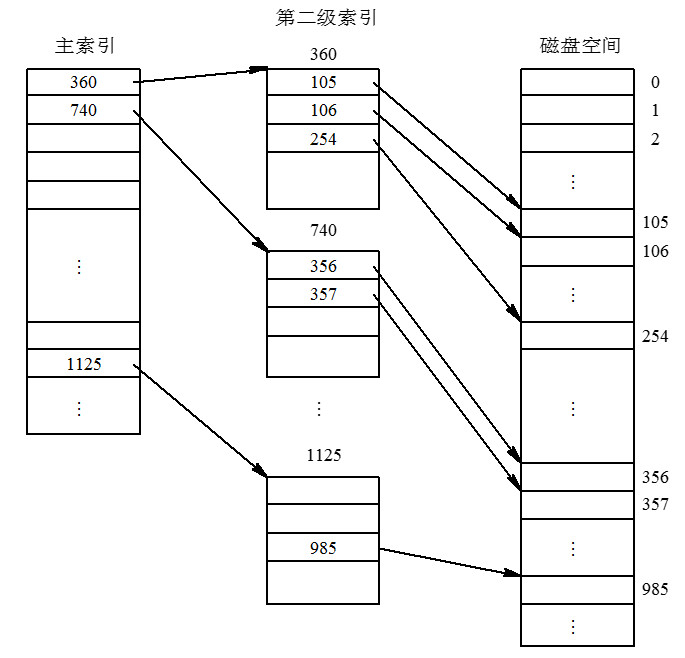
\includegraphics[width=0.6\textwidth]{figure/file/alloc-index2.jpg}
  \end{center}  
\end{frame}

\begin{frame}[fragile]{3. 混合索引分配}
  \begin{center}
    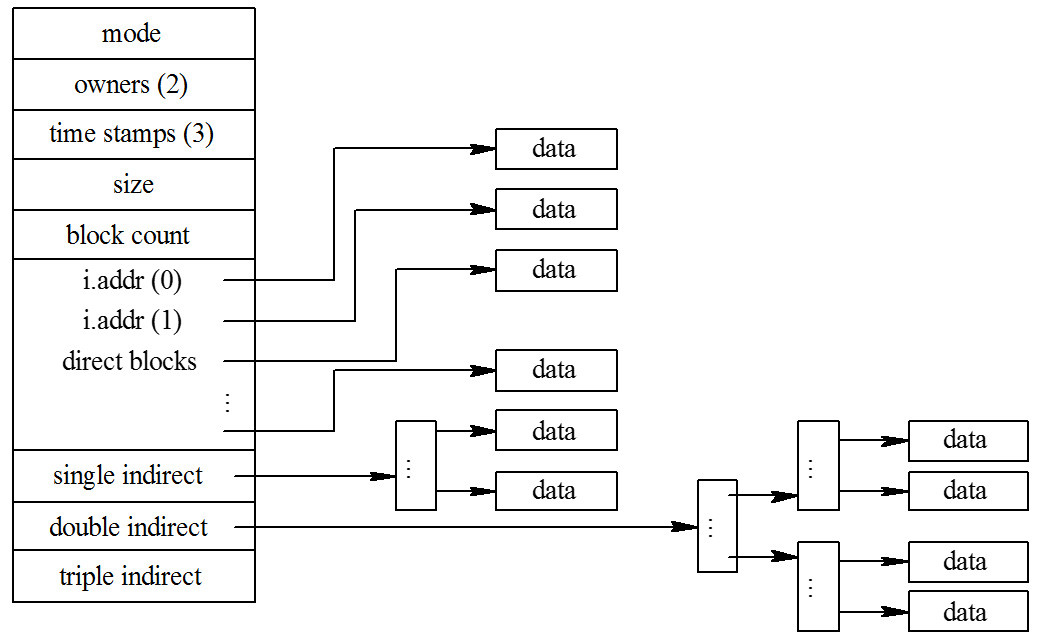
\includegraphics[width=0.8\textwidth]{figure/file/alloc-index3.jpg}
  \end{center}  
\end{frame}


\subsection{6.4 目录管理}
\begin{frame}[fragile]{6.4 目录管理}
  \begin{easylist}
    & 目录管理的要求
    && (1)实现“按名存取”:最基本的功能和服务 
    && (2)提高对目录的检索速度。 
    && (3)文件共享:多用户系统中允许多个用户共享一个文件,只保留一个副本,提供存储利用率,方便用户操作 
    && (4)允许文件重名。
  \end{easylist}
\end{frame}

\begin{frame}[fragile]{6.4.1 文件控制块和索引结点}
  \begin{easylist}
    & 文件控制块
    && 为了能对一个文件进行正确的存取,必须为文件设置用于描述和控制文件的数据结构,称为“文件控制块FCB”
    && 文件与文件控制块一一对应,把文件控制块的有序集合称为文件目录。
    && 一个文件目录也被看成是一个文件,称为目录文件
  \end{easylist}
\end{frame}

\begin{frame}[fragile]{1 文件控制块}
  \begin{easylist}
    & 通常包含三类信息:
    && 基本信息:文件名、文件物理位置、逻辑结构、物理结构
    && 存取控制信息:文件主的存取权限、核准用户的存取权限、一般用户的存取权限
    && 使用信息:文件建立时间、上次修改时间、当前使用信息(已打开文件的进程数、是否锁定、是否被修改尚未拷回磁盘)
  \end{easylist}
\end{frame}

\begin{frame}[fragile]{MS-DOS的文件控制块举例}
  \begin{center}
    \begin{tikzpicture}[c/.style={draw,align=center,minimum height=0.8cm}]
	\draw node[c, minimum width=2.5cm](b1){文件名} 
        node[c,right=0 of b1](b2){扩展名}
        node[c,right=0 of b2](b3){属性} 
        node[c,right=0 of b3, minimum width=2cm](b4){备用} 
        node[c,right=0 of b4](b5){时间} 
        node[c,right=0 of b5](b6){日期} 
        node[c,right=0 of b6](b7){第一块号} 
        node[c,right=0 of b7](b8){盘块数};
      \end{tikzpicture}
  \end{center}
  \begin{easylist}
    & 文件名:8字节
    & 扩展名:3字节
    & 属性:01H—只读、02H—隐含、04H—系统文件、08H—卷标、10H子目录、20H—存档文件。可组合成复合属性,如27H—已存档、系统文件、隐含、只读
    & 时间:2字节,第0~4位:为2x秒(0~29); 第5~10位:分(0~59); 第11~15位:时(0~23)
    & 日期:2字节,第0~4位:日(1~31); 第5~8位:月(1~12); 第9~15位:年(1980年基准)
  \end{easylist}
\end{frame}

\begin{frame}[fragile]{2 索引节点}
  \begin{easylist}
    & 1) 索引结点的引入 
    && 必要性
    &&& 文件目录存放在磁盘上,且可能要占用大量盘块N ,检索开销很大(盘块调入次数 $\dfrac{N+1}{2}$)
    && 可行性
    &&& 只有文件名对目录检索有用,对文件进行描述的信息,在检索时用不到。
  \end{easylist}
\end{frame}

\begin{frame}[fragile]{UNIX方式}
  \begin{easylist}
    & 采用把文件名和文件描述信息分开的办法,使文件描述信息单独形成一个称为索引结点的数据结构,称为i结点。每一个目录仅占16字节,其中14个字节为文件名,2个字节为i结点指针。
  \end{easylist}
  \begin{center}
    \begin{tikzpicture}[a/.style={draw,align=center,minimum height=0.8cm, minimum width=2cm},
      b/.style={draw,align=center,minimum height=0.8cm, minimum width=2.5cm},
      c/.style={draw,align=center,minimum height=0.8cm, minimum width=4cm}]
      \draw node[a, minimum width=2.5cm](a0){文件名} node[b,right=0 of a0](b0){索引结点编号} node[c,right=of b0](c0){文件描述控制信息} 
      node[a, minimum width=2.5cm, below=0 of a0](a1){文件名1} node[b,right=0 of a1](b1){} node[c,right=of b1](c1){} 
      node[a, minimum width=2.5cm, below=0 of a1](a2){文件名2} node[b,right=0 of a2](b2){} node[c,right=of b2](c2){} 
      node[a, minimum width=2.5cm, below=0 of a2](a3){文件名3} node[b,right=0 of a3](b3){} node[c,right=of b3](c3){} ;
      \draw node[below=0.5 of a3, xshift=1.5cm]{UNIX文件目录} node[below=0.5 of c3]{索引结点(i结点)集合};
    \end{tikzpicture}
  \end{center}
  Question: 文件名称有长度限制吗?%Linux文件名称的长度限制是255个字符
\end{frame}

\begin{frame}[fragile]{iNode示意图}
  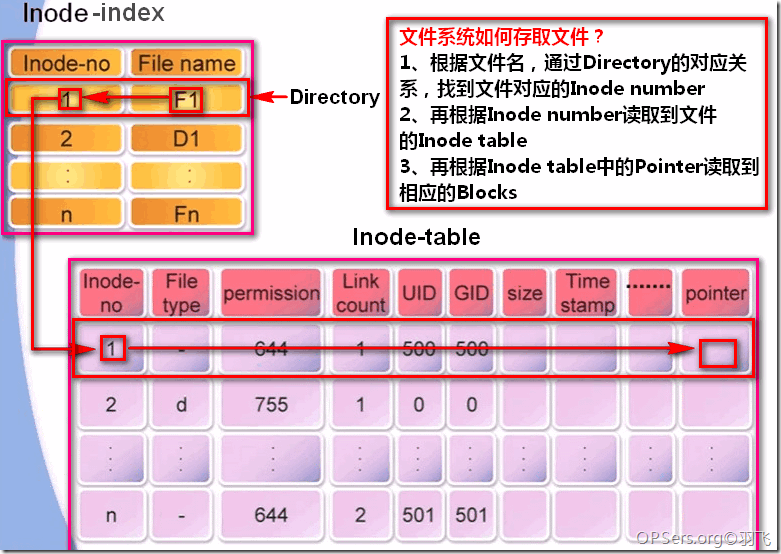
\includegraphics[width=0.9\textwidth]{figure/inode.png}
\end{frame}

\begin{frame}[fragile]{索引结点检索开销分析}
  \begin{easylist}
    & 举例说明
    && 盘块大小1KB,文件目录共3200个FCB
    & 引入索引结点前
    && FCB占64B,每盘块包含16个FCB,文件目录共需占用200个盘块,故查找一个文件平均需启动磁盘100次
    & 引入索引结点后
    && 目录项仅占16B(文件名和索引结点指针分别占用14B和2B),每盘块包含64个目录项,文件目录共需占用50个盘块,故查找一个文件平均需启动磁盘25次
  \end{easylist}
\end{frame}

\begin{frame}[fragile]{磁盘索引节点}
  \begin{easylist}
    & 2) 磁盘索引结点:
    && 存放在磁盘上的索引结点,每个文件有唯一的磁盘索引结点,包括: 
    &&& (1) 文件主标识符:文件拥有者的标识符 
    &&& (2) 文件类型:正规文件、目录文件或特殊文件 
    &&& (3) 文件存取权限 
    &&& (4) 文件物理地址:以直接或间接方式给出数据文件所在盘块的编号 
    &&& (5) 文件长度 
    &&& (6) 文件连接计数:指向该文件的指针计数 
    &&& (7) 文件存取时间:
  \end{easylist}
\end{frame}


\begin{frame}[fragile]{iNode查看: stat test.xml}
  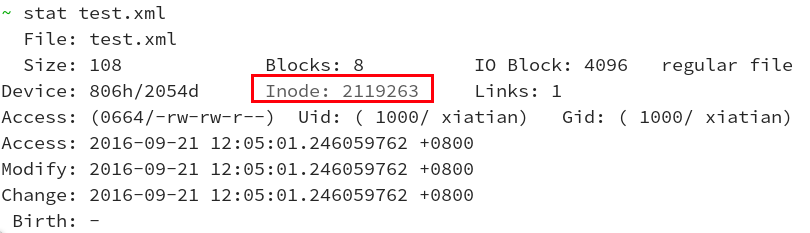
\includegraphics[width=0.9\textwidth]{figure/inode-demo.png}
\end{frame}

\begin{frame}[fragile]{查看系统iNode的总体使用情况}
  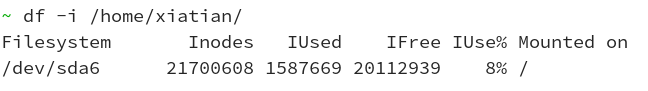
\includegraphics[width=0.9\textwidth]{figure/inode-df.png}
\end{frame}

\begin{frame}[fragile]{inode的特殊作用}
  由于inode号码与文件名分离,这种机制导致了一些Unix/Linux系统特有的现象。
  \begin{itemize}
    
  \item 有时,文件名包含特殊字符,无法正常删除。这时,直接删除inode节点,就能起到
    删除文件的作用。
  \item 移动文件或重命名文件,只是改变文件名,不影响inode号码。
  \item  打开一个文件以后,系统就以inode号码来识别这个文件,不再考虑文件名。因此,
    通常来说,系统无法从inode号码得知文件名。
  \end{itemize}
  
  第3点使得软件更新变得简单,可以在不关闭软件的情况下进行更新,不需要重启。
\end{frame}

\begin{frame}[fragile]{内存索引节点}
  \begin{easylist}
    & 3) 内存索引结点:文件被打开时,将磁盘索引结点拷贝到内存的索引节点中,便于以后使用,内存索引结点又增加如下内容:
    && (1) 索引结点编号:用于标识内存索引结点。
    && (2) 状态:指示i 结点是否上锁或被修改。
    && (3) 访问计数:每当有一进程要访问此i 结点时, 将该访问计数加1,访问完再减1。
    && (4) 文件所属文件系统的逻辑设备号。
    && (5) 链接指针:设置有分别指向空闲链表和散列队列的指针。 
  \end{easylist}
\end{frame}

\begin{frame}[fragile]{6.4.2 目录结构}
  \begin{easylist}
    & 单级目录结构
    & 两级目录结构
    & 多级目录结构
  \end{easylist}
\end{frame}

\begin{frame}[fragile]{1 单级目录结构}
  \begin{easylist}
    & 在整个文件系统中只建立一张目录表,每个文件占一个目录项。
    && 目录项含有文件名、扩展名、长度、类型、物理地址及其他属性信息。同时设置一个状态位表示目录项是否空闲。
    && 新建文件时检索目录项,确保文件名唯一;删除时,回收空间,清除目录项。
  \end{easylist}
  \begin{center}
    \begin{tabular}{|c|c|c|c|}
      \hline
      文件名 & 物理地址 & 文件说明 & 状态位 \\ \hline
      文件名1 & & & \\ \hline
      文件名2 & & & \\ \hline
      $\cdots$ & & & \\ \hline
    \end{tabular}
  \end{center}
\end{frame}

\begin{frame}[fragile]{单级目录结构}
  \begin{easylist}
    & 单级目录的优点是简单且能实现目录管理的基本功能——按名存取,但却存在下述一些缺点:
    && (1) 查找速度慢 
    && (2) 不允许重名 
    && (3) 不便于实现文件共享:无法实现不同用户使用不同文件名来访问同一个文件。 
  \end{easylist}
\end{frame}

\begin{frame}[fragile]{2 两级目录结构}
  \begin{easylist}
    & 为每一个用户建立一个单独的用户文件目录UFD (User File Directory):
    & 在系统中再建立一个主文件目录MFD (Master File Directory)
    && 用户在创建文件时,在自己的用户目录下操作,不同的用户可以拥有同名文件
  \end{easylist}
\end{frame}

\begin{frame}[fragile]{两级目录结构}
  \begin{center}
    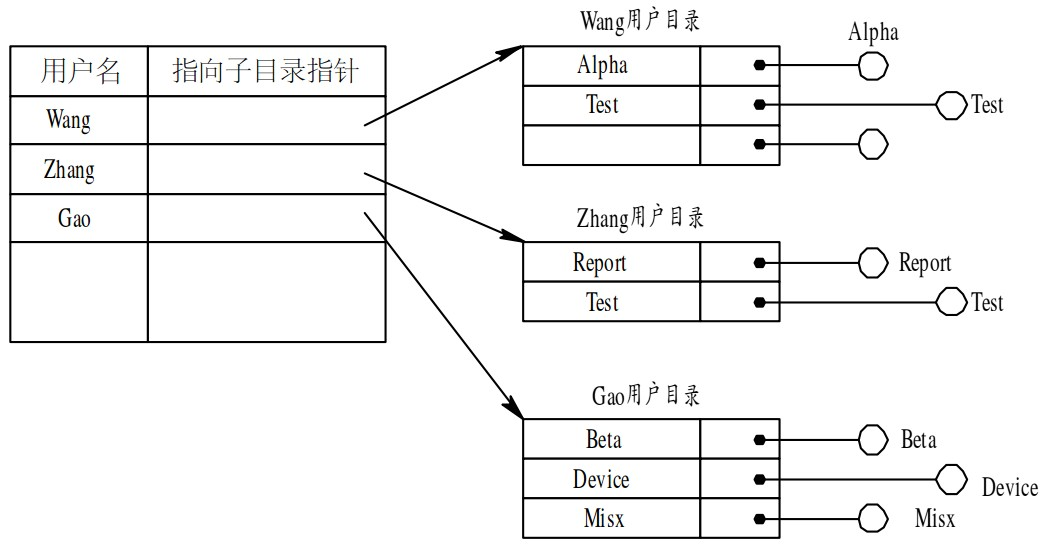
\includegraphics[width=0.8\textwidth]{figure/file/dir-two.jpg}
  \end{center}
\end{frame}

\begin{frame}[fragile]{两级目录结构}
  \begin{easylist}
    & 优点
    && (1)提高了检索目录的速度 
    && (2)在不同的用户目录中,可以使用相同的文件名。 
    && (3)不同用户还可使用不同的文件名来访问系统中的同一个共享文件 
    & 缺点
    && 各用户之间的相互隔离不便于文件的共享,不利于用户之间合作完成一个大任务。
  \end{easylist}
\end{frame}

\begin{frame}[fragile]{3 多级目录结构}
  \begin{easylist}
    & 大型文件系统通常采用三级或以上的目录结构,以提高目录检索速度和文件系统性能。
    & 多级目录结构又称为树型目录结构,主目录称为根目录,数据文件称为树叶。
  \end{easylist}
\end{frame}

\begin{frame}[fragile]{多级目录结构}
  \begin{easylist}
    & (1)目录结构 
  \end{easylist}
  \begin{center}
    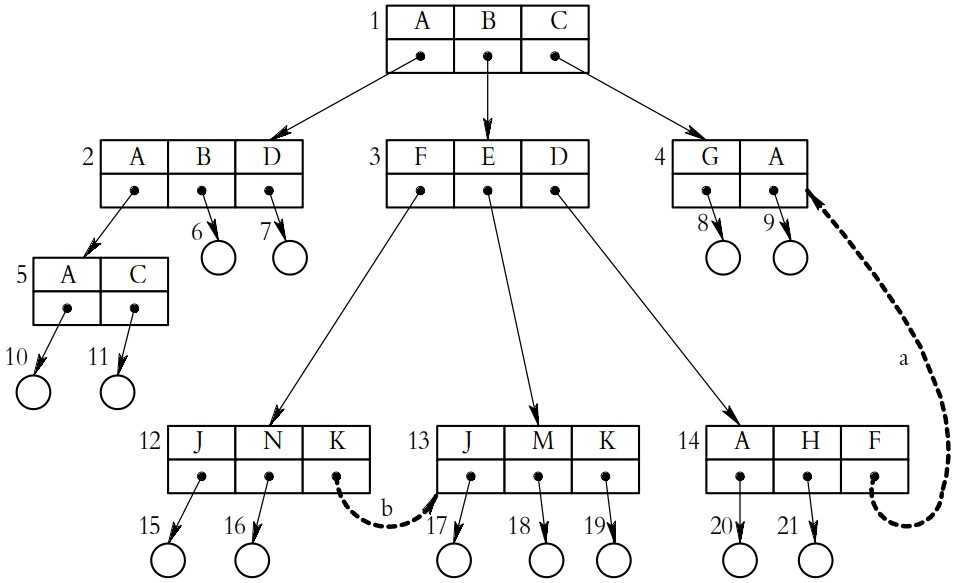
\includegraphics[width=0.8\textwidth]{figure/file/dir-many.jpg}
  \end{center}
\end{frame}

\begin{frame}[fragile]{多级目录结构}
  \begin{easylist}
    & (2)路径名
    && 在树形目录结构中,从根目录到任何数据文件,都只有一条唯一的通路。在该路径上从树的根(即主目录)开始, 把全部目录文件名与数据文件名,依次地用“/”连接起来,即构成该数据文件的路径名(path name)。系统中的每一个文件都有唯一的路径名。
  \end{easylist}
\end{frame}

\begin{frame}[fragile]{多级目录结构}
  \begin{easylist}
    & (3)当前目录(Current Directory)
    && 从当前目录开始直到数据文件为止所构成的路径名,称为相对路径名(relative path name);
    && 从树根开始的路径名称为绝对路径名(absolute path name)。
    && 每个进程当前所在的目录,称为当前目录或工作目录。
    && pwd  command (print work directory)
  \end{easylist}
\end{frame}

\begin{frame}[fragile]{多级目录结构}
  \begin{easylist}
    & (4)增加和删除目录
    && (1)不删除非空目录
    && (2)可删除非空目录

    && rm command
  \end{easylist}
\end{frame}

\begin{frame}[fragile]{6.4.3 目录查询技术}
  \begin{easylist}
    & 当访问一个已存在的文件时,系统首先利用用户提供的文件名对目录进行查询,找出该文件的文件控制块或对应的索引节点;然后根据FCB或索引结点中所记录的文件物理地址,换算出文件在磁盘的物理位置;最后,再通过磁盘驱动程序,将所需文件读入内存。常用的查询方式有:
    && 线性检索法
    && Hash
  \end{easylist}
\end{frame}

\begin{frame}[fragile]{1 线性检索法}
  \begin{easylist}
    & 查找/usr/ast/mbox的步骤
  \end{easylist}
  \begin{center}
    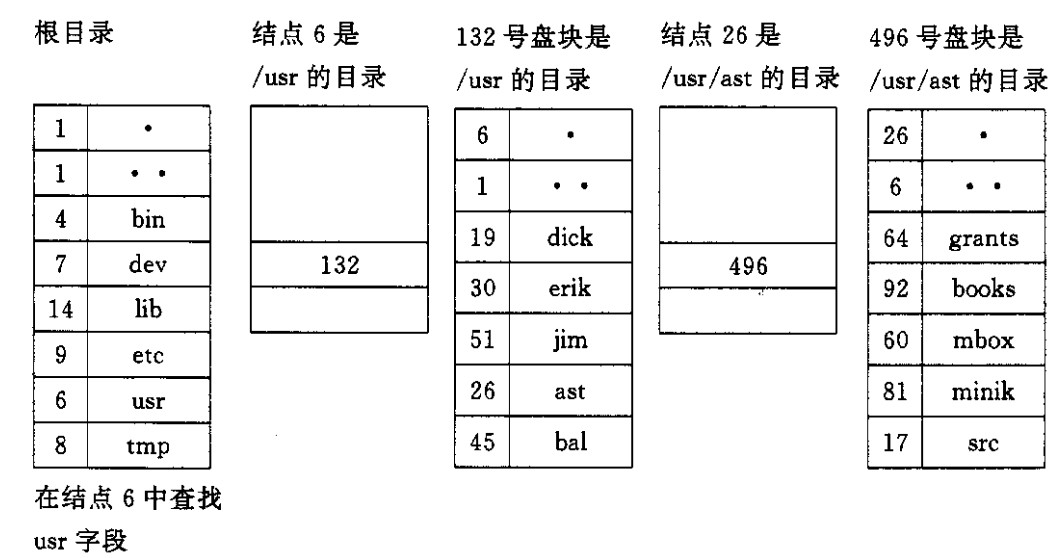
\includegraphics[width=0.8\textwidth]{figure/file/dir-query.jpg}
  \end{center}
\end{frame}

\begin{frame}[fragile]{2 Hash方法}
  \begin{easylist}
    & 处理“冲突”的规则:
    && (1)在利用Hash法索引查找目录时,如果目录表中相应的目录项是空的,则表示系统中并无指定文件。
    && (2)如果目录项中的文件名与指定文件名相匹配,则表示该目录项正是所要寻找的文件所对应的目录项,故而可从中找到该文件所在的物理地址。
    && (3)如果在目录表的相应目录项中的文件名与指定文件名并不匹配,则表示发生了“冲突”,此时须将其Hash值再加上一个常数(该常数应与目录的长度值互质),形成新的索引值,再返回到第一步重新开始查找。
    & “*”, “?”等目录模式匹配问题
  \end{easylist}
\end{frame}

\begin{frame}[fragile]{6.4.4 文件和目录的使用}
  \begin{easylist}
    & 文件访问
    & 文件控制
    & 目录管理
    & 伪文件(Pseudo file)
  \end{easylist}
\end{frame}

\begin{frame}[fragile]{文件访问}
  \begin{easylist}
    & 文件访问是指围绕文件内容读写进行的文件操作。
    && 打开open:为文件读写所进行的准备。给出文件路径,获得文件句柄(file handle),或文件描述符(file descriptor)。需将该文件的目录项读入到内存中。
    && 关闭close:释放文件描述符,把该文件在内存缓冲区的内容更新到外存上。
    && 复制文件句柄dup:用于子进程与父进程间的文件共享,复制前后的文件句柄有相同的文件名、文件指针和访问权限;
  \end{easylist}
\end{frame}

\begin{frame}[fragile]{文件访问}
  \begin{easylist}
    && 读read、写write和移动文件读写指针lseek:系统为每个打开文件维护一个读写指针(read-write pointer),它是相对于文件开头的偏移地址(offset)。读写指针指向每次文件读写的开始位置,在每次读写完成后,读写指针按照读写的数据量自动后移相应数值。
    && 执行exec:执行一个可执行文件;
    && 修改文件的访问模式(fcntl和ioctl):提供对打开文件的控制,如:文件句柄复制、读写文件句柄标志、读写文件状态标志、文件锁定控制、流(stream)的控制;
  \end{easylist}
\end{frame}

\begin{frame}[fragile]{文件控制}
  \begin{easylist}
    & 文件控制是指围绕文件属性控制进行的文件操作。
    && 创建(creat和open):给出文件路径,获得新文件的文件句柄;
    && 删除unlink:对于symbolic link和hard link,删除效果是不同的;
    && 获取文件属性(stat和fstat):stat的参数为文件名,fstat的参数为文件句柄;
    && 修改文件名rename;
    && 修改文件属主chown,修改访问权限chmod:与相应系统命令类似;
    && 文件别名控制:创建symlink或link,读取链接路径readlink;
  \end{easylist}
\end{frame}

\begin{frame}[fragile]{目录管理}
  \begin{easylist}
    & 目录访问和目录属性控制
    && 进行文件访问和控制时,由操作系统自动更新目录内容
    && 目录创建mkdir,删除rmdir,修改目录名rename。只适用于超级用户:mknod(建立文件目录项)和unlink(删除目录项)
    && 更改当前目录chdir;
  \end{easylist}
\end{frame}

\begin{frame}[fragile]{伪文件- pseudo file}
  \begin{easylist}
    & 伪文件是指具有文件某些特征的系统资源或设备,它们的访问和控制方式与文件类似。
    & 特点
    && 内容并不保存在外存上,而是在其他外部设备上或内存里
    && 随文件类型的不同,适用于某些文件访问和控制的系统调用,如:open, read, write, close, chmod, chown。
    && 创建时使用特定的系统调用,如:创建管道pipe,创建管套socket,创建设备文件mknod

    & 类型
    && 设备:字符设备或块设备,可以直接访问设备中的字节数据或数据块。如终端、硬盘、内存等。在UNIX中称为特殊文件(special file)。
    && 进程间通信:本计算机或通过网络。如:管道,管套等。
  \end{easylist}
\end{frame}


\subsection{6.5 文件存储空间的管理}
\begin{frame}[fragile]{6.5 文件存储空间的管理}
  \begin{easylist}
    & 解决如何为新创建的文件分配存储空间,类似于内存的分配,可采用连续或离散分配方式。存储空间的分配单位为磁盘块,而非字节。
    & 为实现存储空间的分配,系统必须能记住磁盘空间的使用情况,应设置响应的数据结构;其次实现对存储空间的分配和回收。
    & 常用的文件存储空间的管理方法:
    && 空闲表法和空闲链表法
    && 位示图法
    && 成组链接法
  \end{easylist}
\end{frame}

\begin{frame}[fragile]{6.5.1 空闲表法和空闲链表法}
  \begin{easylist}
    & 空闲表法
    && 属于连续分配方式,为每个文件分配一块连续的存储空间,系统为外存上的所有空闲区建立一张空闲表。 
  \end{easylist}
  \begin{center}
    \begin{tabular}{|c|c|c|}
      \hline
      序号 & 第一空闲盘块号 & 空闲盘块数 \\ \hline
      1 & 2 & 4 \\ \hline
      2 & 9 & 3 \\ \hline
      3 & 15 & 5 \\ \hline
      4 & --- & --- \\ \hline
    \end{tabular}
  \end{center}
\end{frame}

\begin{frame}[fragile]{空闲表法}
  \begin{easylist}
    & 存储空间的分配与回收
    && 空闲盘区的分配与内存的动态分配类似,同样是采用首次适应算法、循环首次适应算法等
    && 系统在对用户所释放的存储空间进行回收时,也采取类似于内存回收的方法,即要考虑回收区是否与空闲表中插入点的前区和后区相邻接,对相邻接者应予以合并。
    && 对换空间一般采用连续分配方式
  \end{easylist}
\end{frame}

\begin{frame}[fragile]{空闲链表法}
  \begin{easylist}
    & (1)空闲盘块链

    & (2)空闲盘区链 
    && 每个盘区除含有用于指示下一个空闲盘区的指针外,还包含指明本盘区大小的信息。
  \end{easylist}
\end{frame}

\begin{frame}[fragile]{6.5.2 位示图法}
  \begin{easylist}
    & 位示图 
    && 利用二进制的一位表示磁盘中一个盘块的使用情况。所有盘块对应的位构成一个集合,称为位示图
  \end{easylist}
  \begin{center}
    \begin{tabular}{c| c c c c c c c c c c c c c c c c|}
      ~ & 0 & 1 & 2 & 3 & 4 & 5 & 6 & 7 & 8 & 9 & 10 & 11 & 12 & 13 & 14 & 15\\
      \hline
      0 & 1 & 1 & 1 & 1 & 1 & 1 & 1 & 1 & 1 & 1 & 1 & 1 & 1 & 1 & 1 & 1 \\
      1 & 1 & 1 & 1 & 1 & 1 & 1 & 1 & 1 & 1 & 1 & 1 & 1 & 1 & 1 & 1 & 1 \\
      2 & 1 & 1 & 0 & 1 & 1 & 1 & 1 & 1 & 1 & 1 & 1 & 1 & 1 & 1 & 1 & 1 \\
      3 & 1 & 1 & 1 & 1 & 1 & 1 & 0 & 1 & 1 & 1 & 1 & 0 & 1 & 1 & 1 & 1 \\
      4 & 0 & 0 & 0 & 0 & 0 & 0 & 0 & 0 & 0 & 0 & 0 & 0 & 0 & 0 & 0 & 0 \\
      \hline
    \end{tabular}
  \end{center}
\end{frame}

\begin{frame}[fragile]{盘块的分配}
  \begin{easylist}
    & 2.盘块的分配 
    && (1)顺序扫描位示图,从中找出一个或一组其值为“0”的二进制位(“0”表示空闲时)。
    && (2)将所找到的一个或一组二进制位,转换成与之相应的盘块号。假定找到的其值为
    “0”的二进制位,位于位示的第i行、第j列,则其相应的盘块号应按下式计算:  
    $$b=n \cdot (i-1) + j $$
    式中,n代表每行的位数。
    && (3) 修改位示图,令$map[i, j]=1$
  \end{easylist}
\end{frame}

\begin{frame}[fragile]{盘块的回收}
  \begin{easylist}
    & 3.盘块的回收
    && (1)将回收盘块的盘块号转换成位示图中的行号和列号。转换公式为:
    $$ i=(b-1) div  n+1 $$
    $$ j=(b-1) mod n+1 $$

    && (2)修改位示图。令$map[i, j]=0$
  \end{easylist}
\end{frame}

\begin{frame}[fragile]{例}
  \begin{easylist}
    & 有一计算机系统利用如图所示的位示图(行号、列号都从0开始编号)来管理空闲盘块,如果盘块从1开始编号,每个盘块大小为1KB。则:
    && 现要为文件分配两个盘块,试具体说明分配过程。
    && 若要释放磁盘的第300块,应如何处理
  \end{easylist}
  \begin{center}
    \begin{tabular}{c| c c c c c c c c c c c c c c c c|}
      ~ & 0 & 1 & 2 & 3 & 4 & 5 & 6 & 7 & 8 & 9 & 10 & 11 & 12 & 13 & 14 & 15\\
      \hline
      0 & 1 & 1 & 1 & 1 & 1 & 1 & 1 & 1 & 1 & 1 & 1 & 1 & 1 & 1 & 1 & 1 \\
      1 & 1 & 1 & 1 & 1 & 1 & 1 & 1 & 1 & 1 & 1 & 1 & 1 & 1 & 1 & 1 & 1 \\
      2 & 1 & 1 & 0 & 1 & 1 & 1 & 1 & 1 & 1 & 1 & 1 & 1 & 1 & 1 & 1 & 1 \\
      3 & 1 & 1 & 1 & 1 & 1 & 1 & 0 & 1 & 1 & 1 & 1 & 0 & 1 & 1 & 1 & 1 \\
      4 & 0 & 0 & 0 & 0 & 0 & 0 & 0 & 0 & 0 & 0 & 0 & 0 & 0 & 0 & 0 & 0 \\
      \hline
    \end{tabular}
  \end{center}
\end{frame}

\begin{frame}[fragile, allowframebreaks]{计算过程}
  \begin{easylist}
    & A)过程如下:
    && a、顺序检索位示图,找到第一个值为0的二进制位,行号是$i_1=2$,列号$j_1=2$;第二个值为0的二进制位的行号$i_2=3$,列号$j_2=6$。
    && b、计算出找到的两个空闲块的盘块号:
    $$b_1=i_1 \times 16 + j_1 + 1=35 $$
    $$ b_2=i_2 \times 16 + j_2 + 1=55 $$
    && c、修改位示图,令$map[2,2]=map[3,6]=1$,并将35,55分配出去
    \newpage
    & B)过程如下:
    && a、计算出磁盘第300块所对应得二进制位的行号i和列号j:       
    $$ i=(300-1)/16=18; $$
    $$ j=(300-1) \% 16=11$$
    && b、修改位示图,令$map[18,11]=0$
  \end{easylist}
\end{frame}

\begin{frame}[fragile]{6.5.3 成组链接法}
  \begin{easylist}
    & 空闲表法和空闲链表法不适用于大型文件系统。
    & UNIX系统采用了成组链接法,结合了以上两种方法
  \end{easylist}
\end{frame}

\begin{frame}[fragile]{1 空闲盘块的组织}
  \begin{center}
    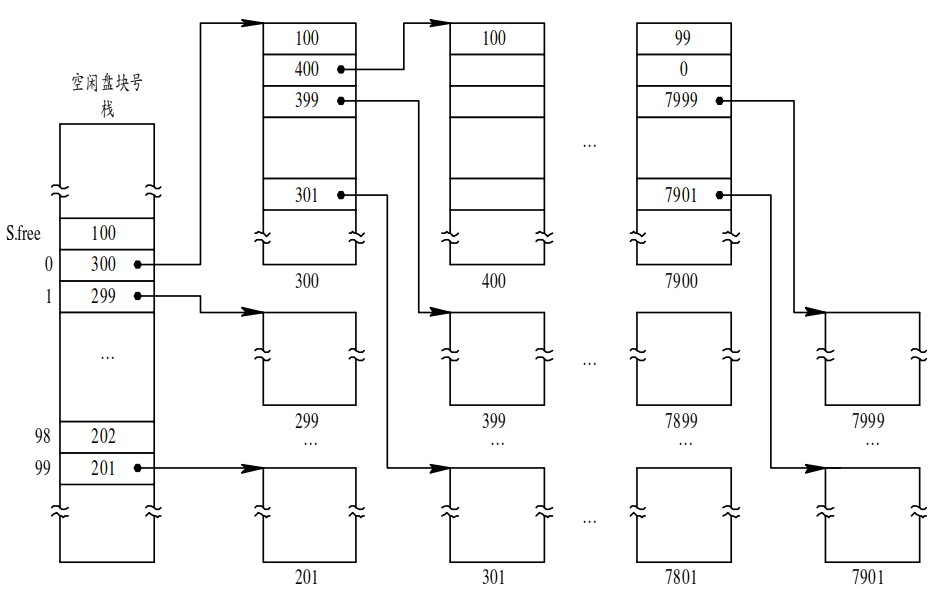
\includegraphics[width=0.8\textwidth]{figure/file/disk-org.jpg}
  \end{center}
\end{frame}

\begin{frame}[fragile]{2 空闲盘块的分配与回收}
  \begin{easylist}
    & 当系统要为用户分配文件所需的盘块时,须调用盘块分配过程来完成。
    && 首先检查空闲盘块号栈是否上锁,如未上锁,便从栈顶取出一空闲盘块号,将与之对应的盘块分配给用户,然后将栈顶指针下移一格。
    && 若该盘块号已是栈底, 即S.free(0),这是当前栈中最后一个可分配的盘块号。由于在该盘块号所对应的盘块中记有下一组可用的盘块号,因此,须调用磁盘读过程,将栈底盘块号所对应盘块的内容读入栈中,作为新的盘块号栈的内容,并把原栈底对应的盘块分配出去(其中的有用数据已读入栈中)。
    && 然后,再分配一相应的缓冲区(作为该盘块的缓冲区)。最后,把栈中的空闲盘块数减1并返回。
  \end{easylist}
\end{frame}

\begin{frame}[fragile]{空闲盘块的分配与回收}
  \begin{easylist}
    & 在系统回收空闲盘块时,须调用盘块回收过程进行回收。它是将回收盘块的盘块号记入空闲盘块号栈的顶部,并执行空闲盘块数加1操作。当栈中空闲盘块号数目已达100时,表示栈已满,便将现有栈中的100个盘块号,记入新回收的盘块中,再将其盘块号作为新栈底。
  \end{easylist}
\end{frame}

\begin{frame}[fragile]{END}
  ~
\end{frame}


%%% Local Variables:
%%% mode: latex
%%% TeX-master: "../os"
%%% End:
